\documentclass{article} % For LaTeX2e
\usepackage{nips14submit_e,times}
\usepackage{hyperref}
\usepackage{url}
\usepackage{amsmath,amsfonts,amsthm}
\usepackage{bbm}
\usepackage{algorithm,algorithmic}
\usepackage{graphicx}
\usepackage{bm}
\usepackage{bbm}
\usepackage[titletoc]{appendix}
\usepackage{wrapfig}
\usepackage{afterpage}
\usepackage{amssymb}

\def\B#1{\bm{#1}}
%\def\B#1{\mathbf{#1}}
\def\trans{\mathsf{T}}

%\renewcommand{\labelitemi}{--}

\newtheorem{theorem}{Theorem} \newtheorem{lemma}[theorem]{Lemma}
\newtheorem{proposition}[theorem]{Proposition}
\newtheorem{corollary}[theorem]{Corollary}
\newtheorem{definition}[theorem]{Definition}
\newtheorem{remark}{Remark}

%%%%%%%%%%%%%%%%%%%%%%%%%%%%%%%%%%%%%%%%%%%%%%%%%%%%%%%%%%%%%%%%%%%%%%%%%%%%%%%

\title{Semi-supervised low-rank logistic regression for
high-dimensional neuroimaging data}


\newcommand{\fix}{\marginpar{FIX}}
\newcommand{\new}{\marginpar{NEW}}
\DeclareMathOperator{\proj}{proj}
\DeclareMathOperator{\soft}{soft}
\DeclareMathOperator{\prox}{prox}
\DeclareMathOperator{\Prox}{Prox}
\DeclareMathOperator{\im}{im}

% macros from michael's .tex
\DeclareMathOperator{\dist}{dist} % The distance.
\DeclareMathOperator{\argmin}{argmin}
\DeclareMathOperator{\argmax}{argmax}
\DeclareMathOperator{\Id}{Id}
\DeclareMathOperator{\abs}{abs}
\newcommand{\R}{\mathbb{R}}
\newcommand{\N}{\mathbb{N}}
\newtheorem{thm}{Theorem}[section]
\newtheorem{prop}[thm]{Proposition}
\newtheorem{lem}[thm]{Lemma}
\newtheorem{cor}[thm]{Corollary}


\nipsfinalcopy % Uncomment for camera-ready version
%%%%%%%%%%%%%%%%%%%%%%%%%%%%%%%%%%%%%%%%%%%%%%%%%%%%%%%%%%%%%%%%%%%%%%%%%%%%%%%

\begin{document}

\author{Danilo Bzdok, Michael Eickenberg, Olivier Grisel,
  Bertrand Thirion,
  Ga\"el Varoquaux \\\\\textbf{\textit{email:} }firstname.lastname@inria.fr}

\maketitle

\begin{abstract}
Imaging neuroscience links human behavior to aspects of brain
biology in ever-increasing datasets.
%
Existing neuroimaging methods typically perform either discovery of
neurobiological structure or evaluation of explicit hypotheses on mental tasks.
%
Modelling mental tasks however hinges
on the pertinence of the assumed neurobiological structure.
%
We therefore propose to solve the unsupervised dimensionality reduction
and supervised task classification in
an identical statistical learning problem.
%
We show that this approach yields more accurate and more interpretable
neural models of psychological tasks in a reference neuroimaging dataset.
%

\textbf{keywords}: dimensionality reduction; semi-supervised learning;
bioinformatics; fMRI; systems neuroscience

\end{abstract}


\section{Introduction}
%
Methods used in neuroimaging research can be grouped by discovering
neurobiological structure or revealing the neural correlates associated
with mental tasks.
To discover coherent distributions of activation structure across time,
independent component analysis (ICA; \cite{beckmann2005}) is often used
to decompose the BOLD (blood-oxygen level-dependent) signals into the
important modes of variation.
The ensuing spatial activation patterns are believed to represent
brain networks of
functionally interacting brain regions.
Similarly, sparse principal component analysis (SPCA; \cite{varoqu2011})
has been used to
separate brain activity signals into parsimonious network components.
Thus extracted brain networks have been shown to be
manifestations of electrophysiological oscillation frequencies \cite{hipp15}.
Their fundamental role in brain organization is
attested by continued covariation during sleep and anesthesia.
%
Network discovery is typically performed by applying ICA or SPCA on
unlabeled "resting-state" data. These capture brain dynamics
during ongoing random thought without controlled environmental input.
The biggest fraction of the BOLD signals are known
not to correlate with a particular behavior, stimulus, or experimental task. 

On the other hand, to investigate
the neural correlates underlying mental tasks,
the general linear model (GLM; \cite{friston94}) is the dominant approach.
The contribution of
individual brain voxels is estimated
according to a design matrix of experimental tasks.
Alternatively, psychophysiological interactions (PPI; \cite{friston97}),
elucidate the functional interactions between voxels as a function
of experimental tasks.
Dynamic causal modeling (DCM; \cite{stephan04}), in turn, quantifies directed,
task-driven influences between regions
by treating the brain as a nonlinear dynamic system with unknown
neuronal states. As a last example, always more neuroimaging studies model
experimental tasks by training classification algorithms on brain signals
\cite{poldrack09decoding}.
All these methods are applied to labeled task data that capture brain dynamics
during stimulus-guided behavior.
Two important conclusions can be drawn.
First, the mentioned supervised neuroimaging analyses operate
without exception in a single-voxel space. This ignores the fact that the BOLD
signal exhibits coherent spatial activation patterns.
Second, existing neuroimaging analyses do not acknowledge the fact that the
task-induced changes of the BOLD signal amount to less than 5\%
of baseline activity \cite{fox07}. They do thus not exploit the high similarity
of BOLD dynamics in the human brain at rest and during experimental tasks.
Indeed, very similar brain networks were observed when applying ICA
separately on rest and task data \cite{smith2009}.

Both biological properties can be conjointly exploited in a 
semi-supervised (i.e., use rest and task data)
low-rank (i.e., perform network decomposition)
approach.
%
The integration of brain-network discovery in a 
supervised classification goal should identify the
neurobiological structure that allows for the best predictive models.
%
Autoencoders suggest themselves because they can emulate
variants of most nonsupervised learning algorithms,
including PCA, SPCA, and ICA.
Autoencoders
are one-layered learning models that condense the input data to
local and global representations
by improving reconstruction from them \cite{hinton06}.
%
They behave like a PCA
in case of one linear hidden layer and a squared error loss
\cite{baldi1989neural}.
This architecture yields a convex optimization objective
with unique global minimum.
Autoencoders behave like a SPCA if shrinkage terms are added for the
matrix weights in the optimization objective.
In turn, they behave like an ICA in case of a nonlinear convex
function of the first-layer activation and tied weights \cite{le2011ica}.
These authors further demonstrated that ICA, sparse autoencoders, and 
sparse coding are mathematically equivalent
under mild conditions.
In this way, autoencoders can flexibly project the neuroimaging data
onto the axes of main variation and thus
reverse-engineer properties of the data-generating
neural processes \cite{olshausen96}.

In the present investigation,
an autoencoder will be fed by (unlabeled) rest data and
integrated as bottleneck
into a low-rank logistic regression fed by (labeled) task data.
Using the chain rule in back-propagation, we can then
solve the unsupervised data representation and a supervised classification
in an identical statistical learning problem.
%
From the perspective of dictionary learning, the first layer can be
viewed as a learned set of basis functions
whose linear combinations are learned
in the second layer \cite{olshausen96}.
%
Neurobiologically, this allows 
delineating a low-dimensional manifold of brain network patterns and then 
distinguishing mental tasks
by their most discriminative linear combinations.
%
Theoretically, a big reduction of the model variance is expected by
regularization using resting-state autoencoder
to put probability mass on the most neurobiologically
valid members of the model space.
%
The generalization performance should consequently be improved due to 
much reduced Vapnik-Chervonenkis dimensions of the classification estimator.
%
Taken together,
the important modes of variation in brain dynamics and
the neural correlates subserving mental operations
have mostly been studied in isolation.
We provide a principled computational framework to link these previously
unconnected domains of systems neuroscience.

\begin{wrapfigure}{r}{0.40\textwidth}
  \begin{center}
    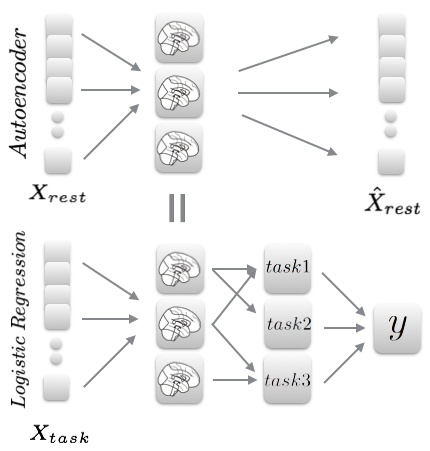
\includegraphics[width=0.40\textwidth]{figures/figure1.png}
  \end{center}
  \caption {\textbf{Architecture}
  }
\end{wrapfigure}

%
\section{Methods}
%
Using
Human Connectome Project (HCP) data (n=500), optimal low-rank projections and
logistic-regression models are identified in a same gradient descent. Brain
network decompositions are thus exposed that explain task-descriminative spatial
patterns.

Data was drawn from 498 unrelated, healthy HCP participants.
All provided informed consent to the Washington
University in St. Louis institutional review board. HCP tasks 
were selected that feature known suitability as localizers
and reliability
across participants \cite{barch2013}.
Mostly block-design, but also event-related, paradigms were
administered on 1) working memory/cognitive control processing, 2)
incentive processing, 3) visual and somatosensory-motor processing,
4) language processing (semantic and phonological processing),
5) social cognition, 6) relational processing, and 7) emotional
processing. All data were acquired on the same Siemens Skyra 3T scanner.
Whole-brain EPI acquisitions were acquired with a
32 channel head coil (TR=720ms, TE=33.1ms, flip angle=52°, BW=2290Hz/Px,
in-plane FOV=$280\times180$mm, 72 slices, 2.0mm isotropic voxels).
The “minimally preprocessed” pipeline \cite{glass13} includes
gradient unwarping, motion correction, fieldmap-based EPI distortion
correction, brain-boundary-based registration of EPI to structural
T1-weighted scan, non-linear (FNIRT) registration into MNI space,
and grand-mean intensity normalization. Activation maps were spatially
smoothed by a Gaussian kernel of 4mm (FWHM). A general linear model (GLM) was
implemented by FILM from the FSL suite with model regressors from convolution
with a “canonical” hemodynamic response function and from temporal derivatives.
HCP tasks were conceived to modulate activation
in a maximum of different brain regions and neural systems. Indeed, at
least 70\% of the participants showed consistent brain activity in
contrasts from the task battery, which certifies excellent
coverage \cite{barch2013}.
In sum, the HCP task dataset incorporated 8650 first-level activity maps
from 18 diverse paradigms administered to 498 participants.
All maps were downsampled to a common 36x43x36 space of
5mm isotropic voxels and gray-matter masked (at least 10\%).
All analyses were based on task maps of
13,657 voxels representing Z values in gray matter.
\linebreak

Unsupervised and supervised learning were combined into a low-rank logistic
regression problem. The 13,657 z values from each activity map were
subject to a first linear
projection into Z latent components (i.e., 1, 5, 10, .., 100).
These hidden brain networks
loadings were subsequently projected into the 18 class space for multinomial
logistic regression. The goal was to find the two weight matrices
(input-to-hidden: 13,657 x Z and hidden-to-output: Z x 18) and their
corresponding bias vectors. Non-linearities were not applied on the
transformation results. Weights and biases were initialized by Gaussian
random noise. Gradient descent updated these matrices and vectors in each
iteration (100 samples per batch, 250 epochs). Using the chain rule, the
partial
derivates for the update were computed for the transformation into the
latent space and the subsequent transformation into the class space. We choose
the RMSprop algorithm \cite{rmsprop} with an initial learning rate of
0.01. Early stopping ensured that the best weight matrices/vectors were
retained in each epoch cycle. This was evaluated by the prediction
accuracy on a validation set (10\% of the training data) at each iteration.
\linebreak

This approach was benchmarked against independent dimensionality reduction and
learning of a classification function. Data reduction was performed on one
half of the data by ICA and SPCA.
ICA unmixed the
BOLD signals into separate spatial components
by minimizing their mutual information \cite{hyvarinen2000}.
This iterative blind source separation was
realized by a parallel FASTICA implementation (200 maximum iterations,
per-iteration tolerance of 0.0001,
initialized by a random mixing matrix, preliminary whitening).
SPCA separated the BOLD signals into
network components with few regions, which scales well to 
large datasets \cite{varoqu2011}.
This regression-type optimization problem constrained by
$\ell_1$-penalty in an implementation
without orthogonality assumptions
(1000 maximum iterations, per-iteration tolerance of 1 * 10\textsuperscript{-8}, sparsity
alpha=1, ridge-shrinkage at 0.01, Lasso path computed with coordinate
descent). Each linear decomposition revealed the specified number of
latent network components in one half the HCP data.
\linebreak
The extracted hidden network components were subsequently used
to reduce the remain half of task maps to a considerably smaller number of component
loadings. 13,657 voxels were thus condensed into 1, 5, 10, .., 100
measures of network involvement using ridge regression
(regularization alpha parameter=0.001, using
Cholesky solver). Multinomial logistic regression was finally performed on the
brain network loadings to learn classifying the 18 cognitive tasks.
Importantly, in all approaches, the final classification models were tested
on an unseen test set (10\% of data).
\linebreak

linear decomposition + elastic net penalty -> has characteristics of a
sparse PCA
\begin{wrapfigure}{r}{0.40\textwidth}
  \begin{center}
    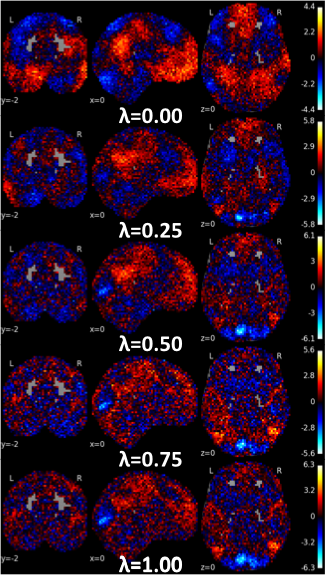
\includegraphics[width=0.40\textwidth]{figures/figure3.png}
  \end{center}
  \caption {\textbf{Equilibrium between autoencoder and low-rank logistic regression}
  One learned decomposition component (out of 20) between the only-autoencoder
  (\textit{uppermost panel}) and only-logistic-regression
  (\textit{lowermost panel}) scenarios.
  The congruent structure (\textit{red, middle column})
  in the
  posterior cingulate cortex, posterior mid-cingulate cortex, and medial
  prefrontal cortex that is hence important in decompositions of the rest and
  task neuroimaging data. With increasing weight on the supervised learning,
  non-congruent structure emerges in the early (\textit{blue}) and
  lateral (\textit{red}) visual cortex
  (\textit{right column}). Matrix weights were z-scored.
  }
\end{wrapfigure}

Learning of the identity function as trivial solution is avoided by
the both bottleneck and the sparsity-enforcing ElasticNet penalty.

o maximize intranetwork homoge- neity and between-network heterogeneity. 


AE:
coordinate system for points on the manifold
low-dimensional bottleneck layer

FORMULA
%X e R^d real-valued input
'reconstruction error' criterion
encoder: input -> hidden reprsentation
%Its parameter set is θ = {W, b}, where W is a d′ × d weight matrix and b is an offset vector of dimensionality d′.
%decoder: gθ′ (y) = s(W′y + b′), (3)
%with appropriately sized parameters θ′ = {W′,b′}.
where b0 and b1 are biase vectors
average reconstruction error
pen. avoids learning trivial soutoin - identitiy

coompute the error derivates of the weights
gradually modified according to possible compression algorithms


affine autoencoder with squared error loss
%tied weights beteen W0 and W1, i.e., W1 = W0^T
X hat is a dterministic function of X
It can thus be said that training an autoencoder to minimize reconstruction error amounts to maximizing a lower bound on the mutual information between input X and learnt repre- sentation Y .

rest data is already compressed to a sparse PCA remote form of 
pretraining of the first layer
bottleneck -> unter-complete representing, i.e. lossy compression

as a pretraining strategy

are decomposed into d networks,
in a way that maximizes the homogeneity of
function within each network while maximizing the heterogeneity between them.

output is vector-valued -> generative properties?
optimal transformation matrix 

forward propegation: input through architecture to generate output
reconstruction cost
backward propegation: generate the deltas for all units / model paramters
corresponds to the derivative of the cost function with respect to the parameters



100 components close to sparse over-complete representation because
Xrest contains only 20 components

whereas elasticnet on the model paramters is regulization

\paragraph{Hints.}
In fact, the constraint by a rest-data autoencoder qualifies as a
\textit{hint} rather than regularization \cite{abu1994hints}.
Its purpose is not to prevent overfitting but to introduce
prior knowledge on known properties of the unknown target function $f$.
Rather than relying only on input-output pairs in the learning process,
we thus narrow our hypothesis set to the biologically most plausible solutions.
That is, we reduce the search space in a way that
is compatible with the expected representation of BOLD activity signals.




FORMULA

\begin{eqnarray}
  \begin{split}
{arg\,min}_\theta \hspace{0.2cm} {\mathcal{L}}(\theta, \lambda) &= \lambda\frac{1}{N_{X_{task}}} \sum_{i=0}^{N_{X_{task}}} \log(P(Y=y^{(i)}|x^{(i)}; W,b)) \hspace{0.2cm} \\
&+ \hspace{0.2cm} (1-\lambda)\frac{1}{N_{X_{rest}}}\|X_{rest}-\hat X_{rest}(W,b)\|^2
  \end{split}
  \label{eq:loss_equ}
\end{eqnarray}

mutiple output units
aCcording to equation \eqref{eq:loss_equ}
As solver, we chose \textit{rmsprop} \cite{rmsprop},
a mini-batch version of rprop.
This procedure dictates an adaptive learning rate
for each model parameter by
scaled gradients from a running average.
Gradient normalization by RMSprop
is known to effectively exploit curvature information.
We opted for a small batch size of $100$, given the high degree of
redundancy in $X_{rest}$ and $X_{task}$.
The matrix parameters were initalized by Gaussian random values multiplied
by a gain of $0.004$. The bias parameters were initalized to be zero.

With a slight abuse of notation, let $\theta$ denote a component of $\theta$.
The normalization factor and the update rule for $\theta$
are given by

\begin{eqnarray}
  \begin{split}
v^{(t+1)} &= \rho v^{(t+1)} + (1 - \rho)\left(\frac{\partial f}{\partial \theta}\right)^2
%v^{(t+1)} = \rho v^{(t+1)} + (1 - \rho)˜|\nabla f
\\
\theta^{(t+1)} &= \theta^{(t)} + \alpha \frac{\nabla f(\theta^{(t)})}{\sqrt{v^{(t+1)} + \epsilon}},
  \end{split}
\end{eqnarray}

where $0 < \rho < 1$ constitutes the decay rate. $\rho$ was set to
$0.9$ to deemphasize the magnitude of the gradient.
Further $\alpha$ is the learning rate and $\epsilon$ a global damping factor.
The hyper-parameter $\alpha$ was set to $0.00001$ by prior manuel
cross-validation and $\epsilon$ was set to $1^{-6}$.
%
Note that we have also experimented with other solvers
(stochastic gradient descent, adadelta, and adagrad) but found that
rmsprop converged faster and with higher generalization performance.

20 components: high bias/low variance
100 compoentens: low bias/high variance

Generating samples from the learned statistical model

minimizing the discrepancy between the orig- inal data and its reconstruction.
The required gradients are easily obtained by using the chain rule to
backpropagate error derivatives first through the decoder network
and then through the encoder network 

theanopython
The analyses were performed in Python.
We used \textit{nilearn} to handle
the high-dimensional neuroimaging data 
\cite{abrah14}
and
\textit{theano} for automatic
differentiation of symbolic computation graphs
\cite{bastien2012theano, bergstra2010theano}.
All Python scripts that generated the results are
accessible online for reproducibility and reuse
\url{http://github.com/banilo/nips2015}.




\section{Experimental Results}


all vectors are column vectors

affine encoder and decoder

Low-rank regression outperformed serial ICA/SparsePCA and logistic regression.

reduction of n gray-matter voxels to n components





Modifications of the mode that di not improve the genralization performacne:
dropo-out, input corruption, addining non-linearities (sigmoid, tanh),


introducing a
nonlinearity (sigmoid, tanh) into the system did not improve predictive accuracy but
elastic did -> most useful decomposition has characteristics of a SPCA
and not PCA or ICA

outperforms plain vanilla LR
inject prior domain knowledge into the learning process





\section{Discussion and Conclusion}
%
There is an increasing occurrence of high-dimensional problems in the
neuroimaging domain. This calls for new statistical learning algorithms that
behave well in large-cohort settings. Ideally, they should acknowledge
and exploit existing widely-accepted neuroscientific knowledge.
In the present work, we propose such an estimator that learns
dimensionality reduction
in a neurobiologically valid and interpretable fashion.

-hypothesis space includes sparse PCA and PCA but not ICA since no
linearity

respect structure in the fMRI data


- if linearity, then would be closer to the notion of 1-hidden layer neural
network rather than low-rank logistic regression



We hope that these results stimulate the development of
even more powerful semi-supervised classification methods


improve computational tractability, prediction accuracy, and interpretability
neuroimaging datasets
does it produce testable predictions?
-> we can test predictive value of network-network architectures across
mental domains.

open window to study the correspondence between brain dynamics during
every-day mind-wandering and task-focused brain states.

classifier that operates in a (sparse) network space, rather than in a voxel space.
domain-specifc classification algorithms

repertoire of mental operations that the human brain can perform

large quantities of neuroimaging data
logistic regression in an autoencoder paradigm

automatically learn a mapping to and from a brain-network space

statistical structure

PCA:
captures structure in the data that is well described by Gaussian clouds,
linear pair-wise correlations are most important form of statistical
dependence/orthongonal components

-> BOLD images can readily be reduced to linear combinations of
sparse spatial structures

scale different classificatiuon architectures to large neuroimaging data

task data might concentrate near a low-dimensional manifold of brain networks

neurobiolgocial fidelity

entities of the neuroimaging domain

There is much uncertainty about the most pertinent representation
of neural activation information
put probability mas shwere we expeted neurobiological strucuture

canonical set of brain networks


FUTURE
link the restings-tate component to the pattern sof cognitive proceses
reduce information von resting-state data in neurological and psychiatric
populations for discovery of neurobiological sub-groups as well as
prediction of disease trajectories and drug responses


%
\paragraph{Acknowledgment}
{\small
Data were provided the Human Connectome Project. The study was supported
by the German National Academic Foundation (D.B.).
}


\small
\bibliographystyle{splncs03}
\bibliography{nips_refs}

\end{document}
